\documentclass[12pt]{article}

\usepackage{sbc-template}
\usepackage{graphicx,url}
\usepackage[utf8]{inputenc}
\usepackage[brazil]{babel}
\usepackage{booktabs}

\sloppy

\title{Avaliação Exploratória de um Modelo Compacto de \emph{Tool-Calling}
para Interfaces de Comando em Português no Contexto de IoT Apícola}

\author{
Renato William Rodrigues de Souza,
Luiz Henrique de Sousa Vieira\\
João Isaac Silva Miranda,
Lívia Pereira Mota\\
Valdenio Mendes Mascena
}

\address{
Instituto Federal de Educação, Ciência e Tecnologia do Ceará (IFCE) - \\ Campus Boa Viagem
}

\begin{document}

\maketitle


\begin{resumo}
Este trabalho apresenta uma avaliação exploratória do Needle 2,
modelo compacto de \textit{tool-calling} com aproximadamente
45 milhões de parâmetros, para interpretar comandos em português
no contexto de IoT apícola. Foram avaliadas 36 solicitações em
um motor de referência executado em host e em um ESP32-S3 N16R8
físico, utilizando o mesmo conjunto de comandos e ferramentas.
Segundo o gabarito histórico, com 33 casos avaliáveis, a
acurácia exata foi de 39,39\% no host e 42,42\% no ESP32-S3.
As sequências de chamadas coincidiram em 34 das 36 solicitações
(94,44\%). No microcontrolador, a latência total média foi
de 35,85~s e a taxa média de geração foi de
1,378~token/s. A reavaliação retrospectiva revelou dificuldades do modelo em reconhecer situações que exigiam abstenção, especialmente diante de comandos ambíguos ou não contemplados pelas ferramentas disponíveis. Embora todas as 36 solicitações tenham sido processadas no ESP32-S3, a geração de chamadas funcionalmente corretas permaneceu limitada. Ressalta-se que o experimento avaliou exclusivamente a interpretação dos comandos e a geração de chamadas estruturadas, sem executar operações sobre sensores ou atuadores.
\end{resumo}



\begin{abstract}
This paper presents an exploratory evaluation of Needle 2,
a compact \textit{tool-calling} model with approximately
45 million parameters, for interpreting Portuguese commands
in an apiculture IoT scenario. We evaluated 36 requests
using both a host reference engine and a physical
ESP32-S3 N16R8, with the same commands and tool definitions.
Under the original reference annotations, which contained
33 evaluable cases, exact-match accuracy was 39.39\%
on the host and 42.42\% on the ESP32-S3.
The two environments produced identical tool-call
sequences for 34 of the 36 requests (94.44\%).
On the microcontroller, mean end-to-end latency was
35.85~s and mean generation throughput was
1.378~tokens/s. A retrospective reassessment revealed difficulties in abstaining from ambiguous or unsupported requests. Although the ESP32-S3 successfully processed all 36 requests, the functional correctness of the generated tool calls remained limited. The experiment was restricted to generating and evaluating structured tool calls, without executing the tools or activating sensors and actuators.
\end{abstract}


\section{Introdução}

Sistemas baseados em Internet da coisas (IoT) permitem monitorar colmeias e reduzir inspeções manuais frequentes \cite{henry2019precision,meikle2015application}. No semiárido, distâncias entre propriedades e conectividade instável dificultam a supervisão remota. Embora painéis web e comandos seriais permitam consultar dados e configurar dispositivos, sua operação pode exigir conhecimentos técnicos pouco acessíveis a alguns produtores.

Modelos de linguagem podem facilitar essa interação, mas a inferência convencional frequentemente exige recursos incompatíveis com microcontroladores ou serviços em nuvem. Modelos compactos de \textit{tool-calling} oferecem uma alternativa local. O Needle 2, divulgado com aproximadamente 45 milhões de parâmetros, é um exemplo dessa abordagem; seus resultados públicos, porém, não estabelecem seu desempenho em português no domínio apícola~\cite{cactusneedle2repo}.

O Needle 2 integra a família de modelos compactos de
\textit{tool-calling} disponibilizada pela Cactus Compute. Segundo
a documentação do projeto, a versão utilizada emprega quantização
CQ2-bit e possui um arquivo de pesos de aproximadamente 14~MB,
com estimativa de cerca de 28~MB de memória para uma sessão de
inferência~\cite{cactusneedle2repo}. Esses valores correspondem
às especificações divulgadas pelos desenvolvedores, não a medições
de consumo de memória realizadas neste estudo. A pesquisa sobre
\textit{Simple Attention Networks} oferece fundamentação arquitetural
relacionada~\cite{ndubuaku2026controlled}, sem que isso implique
atribuir ao Needle 2 todos os componentes descritos em outras
versões da família.

Outros modelos compactos de \textit{function-calling} incluem FunctionGemma (270M) e LFM2.5 (230M). O TinyAgent investiga a especialização de modelos para essa tarefa por meio de \textit{fine-tuning}~\cite{erdogan2024tinyagent}. Esses trabalhos motivam avaliar a geração de chamadas estruturadas por modelos menores em domínios específicos.

A interface avaliada neste trabalho recebe comandos em texto, e não
diretamente em áudio. Embora o hardware utilizado disponha de microfone
integrado, seu uso não faz parte do escopo desta avaliação e é considerado
como possibilidade de trabalho futuro. Soluções como a ESP-SR
\cite{espressif2026espsr} permitem reconhecimento local de palavras-chave
em dispositivos ESP32, mas operam com vocabulários previamente definidos.
Neste trabalho, o interesse está na interpretação de diferentes
formulações textuais em linguagem natural para sua conversão em chamadas
estruturadas de ferramentas.

No contexto da apicultura de precisão, sistemas baseados em sensores
permitem acompanhar variáveis como peso, temperatura e umidade das
colmeias \cite{henry2019precision,meikle2015application,danieli2024precision}.
Neste trabalho, o interesse está na camada de interação com esses sistemas, investigando a conversão de comandos em português em chamadas estruturadas de ferramentas, e não no processamento ou na análise dos sinais coletados. Revisões recentes sobre apicultura de precisão destacam que a adoção dessas tecnologias envolve, além do sensoriamento, aspectos relacionados à usabilidade e à interação com o produtor \cite{danieli2024precision}. Nesse contexto, este trabalho investiga de forma exploratória o uso do Needle 2 como interface local de comando em português para um cenário de IoT aplicado à apicultura. O estudo concentra-se em um cenário ainda pouco explorado: a utilização de um modelo compacto de \textit{tool-calling}, executável em microcontrolador, para interpretar comandos em português associados a operações de monitoramento apícola.

As principais contribuições deste trabalho são:
(1) a definição de um cenário experimental de \textit{tool-calling}
para IoT apícola, composto por três ferramentas e 36 solicitações
em português brasileiro; (2) a avaliação da correção funcional das
chamadas geradas pelo Needle 2, incluindo seleção de ferramentas,
argumentos e abstenção; (3) a execução sistemática das 36 solicitações
em um ESP32-S3 N16R8 físico, com caracterização de latência, taxa de
geração e memória; e (4) a comparação das chamadas produzidas no
motor host de referência e no microcontrolador, incluindo concordância
entre saídas e padrões de erro. A avaliação concentra-se na geração
de chamadas estruturadas: não houve execução de ferramentas sobre
sensores ou atuadores, nem validação em campo com apicultores.
Essas limitações são discutidas na Seção~\ref{sec:discussao}.

O restante deste artigo está organizado da seguinte forma:
a Seção~\ref{sec:metodologia} descreve a proposta, o ambiente experimental, o \textit{schema} de ferramentas, o conjunto de teste e o protocolo de avaliação; a Seção~\ref{sec:resultados} apresenta os resultados quantitativos e qualitativos; a Seção~\ref{sec:discussao} discute as implicações dos resultados e as limitações do trabalho; e a
Seção~\ref{sec:conclusao} apresenta as conclusões.

\section{Metodologia}
\label{sec:metodologia}

\subsection{Proposta}
\label{sec:proposta}

A proposta consiste em utilizar um modelo compacto de
\textit{tool-calling} como camada de interpretação entre comandos em
linguagem natural e operações de um sistema de monitoramento apícola.
Foram definidas três ferramentas representativas de consultas e ações
nesse domínio, mantendo o \textit{schema} reduzido diante do orçamento de
contexto do modelo. A Figura~\ref{fig:fluxo} apresenta o fluxo proposto:
o comando em texto é submetido ao modelo, que pode produzir nenhuma,
uma ou múltiplas chamadas estruturadas de ferramentas, conforme a
solicitação e as operações disponíveis no \textit{schema}.


\begin{figure}[ht]
	\centering
	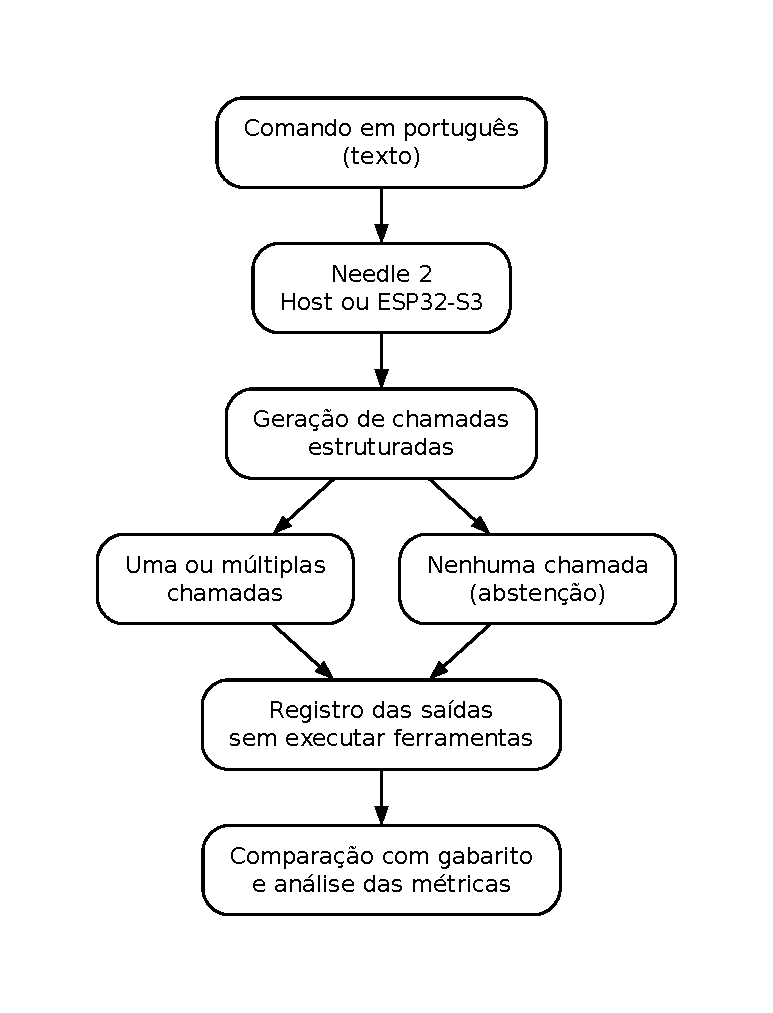
\includegraphics[width=0.6\textwidth]{fluxo_proposta_corrigido.pdf}
	\caption{Fluxo experimental de geração e avaliação de chamadas estruturadas, sem execução de ferramentas.}
	\label{fig:fluxo}
\end{figure}

As operações definidas representam funcionalidades compatíveis com
sistemas de monitoramento apícola baseados em sensores de peso,
temperatura e umidade, entre outras variáveis
\cite{henry2019precision,meikle2015application,danieli2024precision,cota2023bhivesense}. A proposta não modifica a camada de sensoriamento, mas acrescenta uma camada de interação responsável por converter comandos em linguagem natural em chamadas estruturadas de ferramentas.

O protocolo experimental executa a inferência do modelo no host e
no ESP32-S3 físico, mas não despacha as chamadas geradas para
\textit{handlers}. Portanto, não são realizadas consultas a sensores,
operações sobre dados de colmeias ou ações em atuadores, tampouco
execuções de ferramentas com dados simulados. A avaliação concentra-se
na interpretação dos comandos e na correção das chamadas estruturadas
produzidas pelo modelo.


\subsection{Hardware e ambiente}

O ambiente embarcado utilizado foi uma placa ESP32-S3-WROOM-1
N16R8, equipada com 16~MB de memória flash e 8~MB de PSRAM.
O firmware experimental foi desenvolvido utilizando ESP-IDF
v5.4.2 e executou localmente o modelo Needle 2, sem
dependência de serviços externos durante a inferência.

A avaliação considerou dois ambientes de execução.
O primeiro corresponde ao experimento histórico realizado
em Linux, utilizando o motor de referência
\texttt{nd\_dump}. Nesse ambiente, foram processadas
36 frases em português brasileiro, com uma execução
por frase.

O segundo ambiente corresponde à execução sistemática
no ESP32-S3 físico. Foram submetidas ao firmware as
mesmas 36 frases utilizadas no experimento host.
A coleta ocorreu em 25 de outubro de 2026, por meio
da interface serial USB, identificada no ambiente
experimental como \texttt{/dev/ttyACM0}.

O protocolo embarcado utilizou uma sessão persistente
de inferência, com o modelo inicializado antes do
processamento das solicitações. O raciocínio explícito
foi desabilitado mediante o comando \texttt{!think 0},
cuja confirmação foi registrada pelo coletor.
Foram configurados até 96 novos tokens por solicitação
e timeout de 240 segundos por caso.

Os 36 casos foram concluídos, sem registros de casos
incompletos. Os resultados foram obtidos por inferência
real no ESP32-S3, não por simulação ou reprodução
das respostas anteriormente geradas no host.

A avaliação concentrou-se na geração de chamadas
estruturadas de ferramentas. Embora o modelo tenha
produzido comandos associados a operações de
monitoramento e inspeção de colmeias, nenhuma dessas
chamadas foi executada fisicamente sobre sensores
ou atuadores durante o experimento.

Os resultados dos ambientes host e ESP32-S3 foram
registrados separadamente. Essa distinção permite
comparar as chamadas geradas e analisar o desempenho
temporal da execução embarcada, sem atribuir ao
hardware medições realizadas exclusivamente no host.

\subsection{Schema de ferramentas}

O schema foi limitado a três ferramentas para reduzir a ocupação da
janela de contexto documentada para o Needle 2, de 256 tokens
\cite{cactusneedle2repo}:
\texttt{consultar\_status\_colmeia(colmeia\_id)},
\texttt{listar\_colmeias\_alerta()} e
\texttt{ativar\_modo\_inspecao(colmeia\_id, duracao\_min)}. Os nomes dos parâmetros e suas descrições foram definidos com vocabulário
relacionado ao domínio apícola, incluindo termos como peso, temperatura,
alerta e inspeção. O \textit{schema} foi fornecido ao motor em formato
JSON compactado, sem espaços em branco, conforme recomendado pela
documentação do projeto de referência, com o objetivo de reduzir o uso de
tokens de formatação desnecessários.

\subsection{Conjunto de teste}

O conjunto de teste é composto por 36 frases em português brasileiro,
construídas manualmente e associadas previamente às respostas esperadas.
Os casos foram distribuídos em cinco categorias: comandos diretos (N=8);
variações de fala coloquial e numerais por extenso (N=8); parâmetros
ausentes ou vagos (N=6), destinados a verificar se o modelo evita
preencher argumentos não fundamentados no comando; frases ambíguas
(N=6), incluindo referências a múltiplas colmeias, referências espaciais
sem identificador numérico e solicitações mais específicas do que as
operações disponíveis; e frases fora de escopo (N=8), para as quais se
espera uma chamada de ferramenta vazia.

As categorias foram definidas para representar diferentes níveis de
complexidade de interpretação e incluir casos limite relevantes para a
avaliação. Os casos com parâmetros ausentes, ambiguidades e entradas fora
de escopo permitem avaliar, além da seleção da ferramenta, a capacidade
do modelo de evitar argumentos não fundamentados e chamadas indevidas.


\subsection{Protocolo experimental e métricas}

Foram avaliadas as mesmas 36 frases em português brasileiro, uma vez por ambiente: Linux host, com \texttt{nd\_dump}, e ESP32-S3 físico. O limite de geração foi de 96 novos tokens por solicitação, com raciocínio explícito desabilitado. Os tempos máximos foram de 300~s no protocolo histórico do host e 240~s no ESP32-S3. Temperatura, \textit{top-k} e \textit{top-p} não constam do manifesto histórico e não são presumidos. As saídas dos dois ambientes foram registradas separadamente.

A métrica principal de correção funcional foi a
correspondência exata (\textit{exact match}) entre a
sequência de chamadas produzida pelo modelo e a
sequência esperada no gabarito. A comparação considera
os nomes das ferramentas, a quantidade de chamadas
e os respectivos argumentos. Uma abstenção correta
corresponde à ausência de chamadas quando nenhuma
operação é suficientemente determinada ou suportada
pelo contrato de ferramentas.

O gabarito histórico apresentou três casos sem
representação avaliável da resposta esperada
(casos 19, 23 e 25). Por esse motivo, a avaliação
funcional original utiliza 33 casos avaliáveis,
preservando os 36 registros de inferência. Os casos
não avaliáveis não são automaticamente classificados
como erros do modelo.

Uma auditoria posterior identificou inconsistências
adicionais no gabarito histórico, incluindo casos
em que a resposta esperada omitia argumentos
obrigatórios do \textit{schema}. Foi então elaborado
um gabarito revisado, com 36 respostas esperadas
estruturalmente compatíveis com o contrato das
ferramentas. Os resultados obtidos com esse gabarito
constituem uma reavaliação retrospectiva das saídas
já coletadas, não um novo experimento nem uma
substituição silenciosa do protocolo original.

Além da acurácia funcional, foram consideradas a
concordância exata entre as chamadas geradas nos
dois ambientes e a conformidade estrutural das
chamadas com o \textit{schema}. A conformidade
estrutural verifica a presença de ferramentas
reconhecidas e argumentos obrigatórios válidos,
mas não implica correção semântica da resposta.

Para o ESP32-S3, foram analisados os tempos de
processamento registrados durante a execução real,
incluindo latência total por solicitação, tempo de
\textit{prefill}, tempo de geração e taxa de geração
de tokens. Também foram examinados os registros
de memória disponibilizados pelo firmware.
Essas medições caracterizam exclusivamente o
ambiente embarcado e não são inferidas a partir
dos tempos observados no host.

Como cada frase foi executada apenas uma vez em
cada ambiente, o estudo não permite estimar a
variabilidade entre repetições. A comparação
pareada dos acertos foi complementada pelo teste
exato de McNemar, interpretado de forma exploratória,
sem pressupor equivalência entre os ambientes
na ausência de diferença estatisticamente
significativa.

Nenhuma chamada produzida pelo modelo foi
executada fisicamente sobre sensores ou
atuadores. A avaliação concentrou-se na
interpretação dos comandos e na geração
das chamadas estruturadas correspondentes.


\section{Resultados}
\label{sec:resultados}

\subsection{Correção funcional e concordância entre ambientes}

A avaliação compreendeu 36 solicitações em português
brasileiro, executadas uma vez no host e uma vez no
ESP32-S3. No gabarito histórico, três solicitações
(casos 19, 23 e 25) não possuíam respostas esperadas
avaliáveis. Consequentemente, a acurácia funcional
histórica foi calculada sobre 33 casos.

O motor host apresentou 13 acertos em 33 casos
avaliáveis (39,39\%), enquanto a execução real no
ESP32-S3 apresentou 14 acertos (42,42\%). A
Tabela~\ref{tab:metricas} apresenta os resultados
por categoria.

\begin{table}[ht]
\centering
\caption{Correção funcional por categoria, segundo o
gabarito histórico.}
\label{tab:metricas}
\begin{tabular}{lccc}
\toprule
Categoria & Avaliáveis & Host & ESP32-S3 \\
\midrule
Diretos & 8 & 6/8 & 6/8 \\
Variações de fala & 8 & 3/8 & 3/8 \\
Parâmetro implícito & 5 & 1/5 & 1/5 \\
Ambíguos & 4 & 1/4 & 1/4 \\
Fora de escopo & 8 & 2/8 & 3/8 \\
\midrule
\textbf{Total} & \textbf{33} &
\textbf{13/33} & \textbf{14/33} \\
\bottomrule
\end{tabular}
\end{table}

As sequências de chamadas produzidas nos dois
ambientes foram idênticas em 34 das 36 solicitações
(94,44\%). As divergências ocorreram nos casos
6 e 34. No caso 6, o ESP32-S3 produziu uma
chamada adicional de inspeção, além da chamada
observada no host. No caso 34, referente a uma
solicitação fora do escopo das ferramentas, o
host gerou uma chamada indevida, enquanto o
ESP32-S3 não produziu chamadas.

Entre os 33 casos avaliáveis pelo gabarito
histórico, houve 13 acertos simultâneos,
um acerto exclusivo do ESP32-S3 e nenhum
acerto exclusivo do host. O teste exato de
McNemar apresentou $p=1{,}000$, sem evidência
de diferença estatisticamente significativa
na amostra observada. Esse resultado não
estabelece equivalência entre os ambientes.

\subsection{Desempenho da execução embarcada}

A coleta real no ESP32-S3 concluiu as 36
solicitações previstas, sem casos incompletos.
Todas as 36 saídas tiveram chamadas estruturadas
extraídas em formato JSON válido. Isso não
implica correção funcional das respostas.

A latência total média observada foi de
35,85~s, com desvio-padrão de 10,48~s e
mediana de 34,04~s. Os tempos médios
registrados para \textit{prefill} e geração
foram, respectivamente, 14,60~s e 18,15~s.
A taxa média de geração foi de
1,378~token/s.

A Tabela~\ref{tab:desempenho_esp32}
resume as principais medições.

\begin{table}[ht]
\centering
\caption{Desempenho observado no ESP32-S3
em 36 solicitações.}
\label{tab:desempenho_esp32}
\begin{tabular}{lr}
\toprule
Métrica & Valor \\
\midrule
Latência total média & 35,85~s \\
Latência total mediana & 34,04~s \\
Desvio-padrão da latência & 10,48~s \\
Tempo médio de \textit{prefill} & 14,60~s \\
Tempo médio de geração & 18,15~s \\
Taxa média de geração & 1,378~token/s \\
Tokens gerados por solicitação (média) & 25,06 \\
\bottomrule
\end{tabular}
\end{table}

Foram identificadas 35 chamadas de ferramentas
nas 36 respostas embarcadas. Todas as 35
chamadas apresentaram conformidade estrutural
com as ferramentas e os argumentos obrigatórios
do contrato utilizado. Entretanto, a
conformidade estrutural não implica que a
ferramenta selecionada ou seus argumentos
sejam semanticamente adequados à solicitação.

Os registros de memória livre antes e após
cada solicitação não evidenciaram redução
líquida nas medições correspondentes de PSRAM
e memória interna. Essa observação não
permite concluir ausência de fragmentação,
vazamentos transitórios ou outros problemas
de gerenciamento de memória.

\subsection{Reavaliação retrospectiva do gabarito}

Uma auditoria posterior ao experimento
identificou inconsistências no gabarito
histórico. Foram revisadas oito respostas
esperadas, preservando integralmente as
36 frases originais e os registros de
inferência dos dois ambientes.

O gabarito revisado contém 36 casos
estruturalmente avaliáveis. Aplicado
retrospectivamente às saídas já coletadas,
resultou em 13 acertos no host
(36,11\%) e 14 no ESP32-S3
(38,89\%).

Na versão revisada, 17 solicitações
exigiam abstenção, isto é, ausência de
chamadas de ferramentas. O host produziu
chamadas indevidas em 15 desses casos,
enquanto o ESP32-S3 apresentou esse
comportamento em 14 casos. A elevada
frequência de chamadas não solicitadas
indica uma limitação relevante para
interfaces que possam acionar dispositivos
físicos.

O caso 23 ilustra a importância da
auditoria do gabarito. A solicitação
referente às colmeias 3 e 4 produziu
duas chamadas de consulta compatíveis
com a intenção expressa. O gabarito
histórico não continha uma resposta
avaliável para esse caso, enquanto o
gabarito revisado passou a reconhecer
as duas chamadas como resposta correta.

Os resultados retrospectivos são
apresentados como análise complementar
e não substituem a avaliação histórica.


\section{Discussão}
\label{sec:discussao}

\subsection{Interpretação da correção funcional}

Os resultados evidenciam limitações do checkpoint avaliado
na interpretação de comandos em português relacionados à
IoT apícola. Segundo o gabarito histórico, os comandos
diretos apresentaram seis acertos em oito solicitações
(75,0\%) nos dois ambientes. Nas categorias envolvendo
parâmetros implícitos e ambiguidades, os resultados foram
inferiores, com um acerto em cinco e um em quatro casos
avaliáveis, respectivamente.

A reavaliação retrospectiva reforçou a importância de
distinguir a geração de chamadas estruturalmente válidas
da decisão de executar uma ferramenta. Embora todas as
35 chamadas produzidas no ESP32-S3 fossem compatíveis
com a estrutura do contrato utilizado, apenas 14 das
36 respostas foram funcionalmente corretas segundo o
gabarito revisado.

Entre as 17 solicitações que exigiam abstenção nesse
gabarito, o modelo gerou chamadas indevidas em 15 casos
no host e 14 no ESP32-S3. Esse comportamento é
especialmente relevante em sistemas de IoT, nos quais
uma interpretação inadequada pode resultar em ações
não pretendidas caso a execução seja autorizada
sem validações adicionais.

Os resultados são compatíveis com a hipótese de que
a interpretação linguística e a transferência para
um domínio específico representem desafios para o
modelo. Entretanto, o desenho experimental não
permite isolar efeitos do idioma, do domínio ou da
capacidade do modelo. Comparações com conjuntos
equivalentes em outros idiomas e avaliações com
adaptação ao domínio seriam necessárias para
investigar essas hipóteses.

\subsection{Comparação entre host e ESP32-S3}

A concordância exata de 34 das 36 sequências de
chamadas (94,44\%) indica que os dois ambientes
produziram resultados predominantemente iguais
para as solicitações avaliadas. As divergências
observadas ocorreram nos casos 6 e 34.

A avaliação funcional histórica apresentou
13 acertos em 33 casos avaliáveis no host
(39,39\%) e 14 no ESP32-S3 (42,42\%).
O teste exato de McNemar não identificou
diferença estatisticamente significativa
($p=1{,}000$). Considerando o pequeno
conjunto de teste e a ausência de repetições,
não é possível concluir superioridade ou
equivalência entre os ambientes.

A execução local das 36 solicitações no ESP32-S3 confirmou a viabilidade técnica da inferência embarcada nessa configuração. Entretanto, a latência média de 35,85~s e a taxa de geração de 1,378~token/s indicam restrições para interfaces que exijam respostas rápidas. A adequação temporal não foi avaliada com usuários finais.

\subsection{Implicações para IoT apícola}

Os resultados sugerem que a integração de
modelos compactos de \textit{tool-calling}
a sistemas embarcados deve considerar
mecanismos adicionais de segurança.

A validação estrutural de nomes de ferramentas
e argumentos é necessária, mas insuficiente
para garantir a adequação da operação
solicitada. Em particular, comandos ambíguos,
parâmetros obrigatórios ausentes e solicitações
fora do escopo exigem políticas explícitas
de abstenção ou confirmação antes de qualquer
acionamento físico.

No experimento realizado, nenhuma chamada
foi executada sobre sensores ou atuadores.
Assim, os resultados demonstram a geração
local de comandos estruturados, mas não
validam o funcionamento de uma cadeia
completa de controle físico de colmeias.

\subsection{Limitações}

O estudo possui limitações relevantes.
Primeiro, o conjunto contém apenas 36
frases construídas manualmente, sem
validação com apicultores ou revisão
independente por múltiplos anotadores.

Segundo, cada frase foi executada uma
única vez em cada ambiente, impedindo
a estimativa da variabilidade entre
execuções e restringindo a interpretação
da comparação estatística.

Terceiro, o gabarito histórico apresentou
três casos não avaliáveis e outras
inconsistências de especificação. A
revisão posterior foi documentada e
analisada separadamente, mas não equivale
a uma avaliação prospectiva independente.

Quarto, a execução embarcada foi realizada
em uma configuração específica de
ESP32-S3, sem comparação com outros
microcontroladores, configurações de
memória ou estratégias de otimização.

Quinto, não houve integração com sensores
ou atuadores reais, tampouco avaliação
de usabilidade com operadores do
domínio apícola.

Por fim, foi utilizado o checkpoint
público do modelo, sem adaptação
específica ao português ou ao
vocabulário do domínio. Essas
restrições caracterizam os resultados
como exploratórios e limitam sua
generalização para aplicações reais.

\section{Conclusão}
\label{sec:conclusao}

Este trabalho apresentou uma avaliação
exploratória do modelo compacto Needle 2
como mecanismo de interpretação de
comandos em português para IoT apícola,
comparando sua execução em Linux host
e em um ESP32-S3 físico.

Foram processadas 36 solicitações em
cada ambiente. Segundo o gabarito
histórico, que continha 33 casos
avaliáveis, a acurácia funcional foi
de 39,39\% no host e 42,42\% no
ESP32-S3. As chamadas estruturadas
foram idênticas em 34 das 36
solicitações, sem evidência de
diferença estatisticamente
significativa entre os acertos
pareados.

A execução embarcada concluiu todos
os casos previstos, apresentando
latência total média de 35,85~s e
taxa média de geração de
1,378~token/s. Apesar da conformidade
estrutural das chamadas produzidas,
a correção funcional permaneceu
limitada, especialmente em
solicitações que exigiam abstenção.

Os resultados demonstram a
possibilidade de executar localmente
o modelo e gerar comandos estruturados
em um microcontrolador, mas não
sustentam seu emprego autônomo
para acionamento físico de
dispositivos no cenário avaliado.

Como trabalhos futuros, pretende-se
ampliar o conjunto de comandos,
realizar execuções repetidas,
obter avaliação de especialistas
do domínio, investigar estratégias
de adaptação ao português e
otimizar o desempenho embarcado.
A integração controlada com
sensores e atuadores deverá
ser acompanhada de mecanismos
de validação semântica,
abstenção e confirmação
das operações propostas.

\bibliographystyle{sbc}
\bibliography{referencias}

\end{document}
